\title{Aula 8 - Números Pseudoaleatórios}

\author{Prof. Gabriel Rodrigues Caldas de Aquino}

\institute
{
    Instituto de Computação \\
    Universidade Federal do Rio de Janeiro\\
    gabrielaquino@ic.ufrj.br% Your institution for the title page
}
\date{Compilado em: \\ \today} % Date, can be changed to a custom date

%----------------------------------------------------------------------------------------
%    PRESENTATION SLIDES
%----------------------------------------------------------------------------------------



\begin{frame}
    % Print the title page as the first slide
    \titlepage
\end{frame}

\begin{frame}{Geração de Números Aleatórios em Criptografia}
\textbf{Função importante:} geração de números pseudoaleatórios criptograficamente fortes.

\medskip
\begin{itemize}
    \item Os \textbf{Geradores de Números Pseudoaleatórios (PRNGs)} são essenciais para aplicações de criptografia e segurança.
    \item Eles produzem sequências de números que parecem aleatórias, mas são geradas a partir de um estado inicial (\textit{seed}).
\end{itemize}

\medskip
\textbf{Importância dos números aleatórios:}
\begin{itemize}
    \item Garantir \textbf{confidencialidade} em criptografia de chave simétrica.
    \item Produzir \textbf{nonces}, IVs e chaves seguras.
    \item Evitar padrões previsíveis que possam ser explorados por atacantes.
    \item Fundamentais para diversas aplicações de segurança em redes.
\end{itemize}
\end{frame}

\begin{frame}{Uso de Números Aleatórios em Segurança de Redes}
\textbf{Função:} garantir a segurança em diversos algoritmos criptográficos por meio de números binários aleatórios.

\medskip
\begin{itemize}
    \item \textbf{Distribuição de chaves e autenticação mútua:}
    \begin{itemize}
        \item Protocolos cooperativos trocam mensagens para distribuir chaves e autenticar participantes.
        \item \textbf{Nonces} são usados durante o handshaking para evitar ataques de replay.
        \item Números aleatórios nos nonces impedem que atacantes adivinhem ou reutilizem transações antigas.
    \end{itemize}
    
    \item \textbf{Geração de chave de sessão:}
    \begin{itemize}
        \item Chaves temporárias para criptografia simétrica, válidas apenas durante uma sessão.
        \item Aumenta a segurança limitando a exposição da chave.
    \end{itemize}

    \item \textbf{Geração de chaves para RSA:}  
    Números aleatórios são essenciais para gerar chaves de criptografia assimétrica seguras.

    \item \textbf{Fluxos de bits para cifragem de fluxo:}  
    Algoritmos de cifra de fluxo dependem de números aleatórios para criar sequências criptograficamente seguras.
\end{itemize}
\end{frame}

\begin{frame}{Exemplo: VeraCrypt 
tem necessidade de Números Aleatórios}

\centering
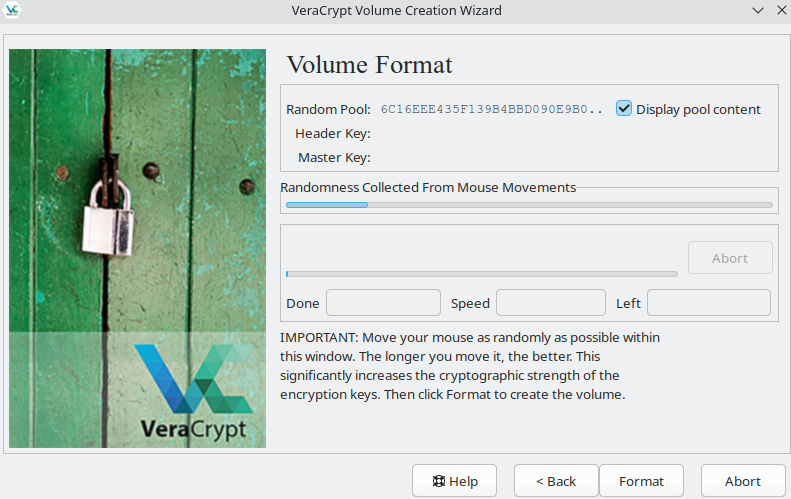
\includegraphics[width=0.8\linewidth]{Figuras/veracrypt-randomness.png}


\end{frame}

\begin{frame}{Critérios para Números Aleatórios}
Tradicionalmente, a preocupação na geração de uma sequência de números supostamente aleatórios é garantir que a sequência seja estatisticamente aleatória.  

\medskip
Dois critérios principais são usados para validar a aleatoriedade:

\begin{itemize}
    \item \textbf{Distribuição uniforme:}  
    A frequência de ocorrência de uns e zeros deve ser aproximadamente a mesma, garantindo que não haja viés.
    
    \item \textbf{Independência:}  
    Nenhum valor na sequência pode ser deduzido a partir dos outros; cada elemento é estatisticamente independente dos demais.
\end{itemize}

\end{frame}

\begin{frame}{Testando Independência de Sequências Aleatórias}
Embora existam testes bem definidos para verificar se uma sequência de bits segue uma distribuição específica, como a \textbf{uniforme}, não há um teste único para \textbf{provar independência}.

\medskip
Estratégia geral:

\begin{itemize}
    \item Aplicar diversos testes estatísticos que verificam propriedades relacionadas à independência.
    \item Se nenhum teste indicar dependência, podemos ter um \textbf{alto nível de confiança} de que a sequência é independente.
    \item A confiança aumenta com o número e a variedade de testes aplicados.
\end{itemize}

\end{frame}


\begin{frame}{Imprevisibilidade em Números Aleatórios}
Em aplicações como autenticação recíproca, geração de chaves de sessão e cifras de fluxo, o requisito principal não é a aleatoriedade estatística, mas a \textbf{imprevisibilidade} dos números sucessivos.

\medskip
\begin{itemize}
    \item Números verdadeiramente aleatórios: cada elemento é independente e, portanto, imprevisível.
    \item Limitações dos números verdadeiramente aleatórios: ineficiência e dificuldade de geração.
    \item Solução comum: algoritmos geradores de números pseudoaleatórios (\textbf{PRNGs}) que aparentam aleatoriedade.
    \item Importante: garantir que um atacante não consiga prever elementos futuros da sequência a partir dos anteriores.
\end{itemize}

\end{frame}

\begin{frame}{Geradores de números aleatórios e pseudoaleatórios}

\centering
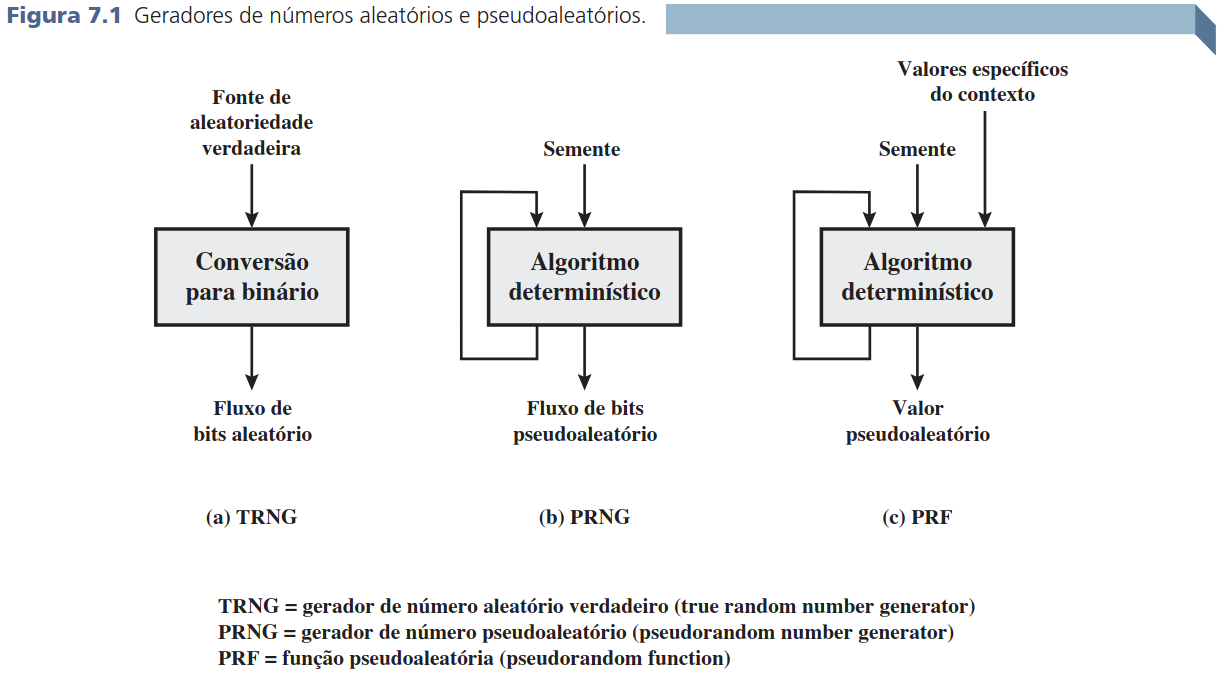
\includegraphics[width=0.9\linewidth]{Figuras/TRNgsPRNGsPRFs.png}


\end{frame}

\begin{frame}{TRNGs, PRNGs e PRFs}
\textbf{Geração de números aleatórios em criptografia:} normalmente realizada por algoritmos determinísticos.

\medskip
\begin{itemize}
    \item \textbf{Determinismo:} Algoritmos produzem sequências que não são estatisticamente aleatórias.
    \item \textbf{Números pseudoaleatórios:} Se o algoritmo for bom, a sequência resultante passa em muitos testes de aleatoriedade.
    \item \textbf{Prática aceita:} Apesar de serem determinísticos, PRNGs funcionam “tão bem quanto” números aleatórios em aplicações criptográficas.
    \item \textbf{Analogias estatísticas:} Semelhante a amostras de uma população — resultados aproximam os da população inteira.
\end{itemize}

\end{frame}

\begin{frame}{TRNG: Geração de Números Aleatórios}
\textbf{Geradores de números aleatórios verdadeiros (TRNG):}
\begin{itemize}
    \item Usam uma fonte efetivamente aleatória, chamada \textbf{fonte de entropia}.
    \item Fontes de entropia podem incluir:
    \begin{itemize}
        \item Padrões de temporização dos toques de tecla.
        \item Movimentos do mouse.
        \item Atividade elétrica no disco.
        \item Valores instantâneos do clock do sistema.
    \end{itemize}
    \item A fonte de entropia serve como entrada para um algoritmo que gera saída binária aleatória.
    \item Pode envolver conversão de sinais analógicos e processamento adicional para eliminar tendências.
\end{itemize}



\end{frame}

\begin{frame}{TRNG vs PRNG}
\begin{block}{TRNG – True Random Number Generator}
A fonte de entropia é retirada do ambiente físico do computador e pode incluir:
\begin{itemize}
    \item Padrões de temporização dos toques de tecla
    \item Atividade elétrica no disco
    \item Movimentos do mouse
    \item Valores instantâneos do clock do sistema
\end{itemize}
A saída é binária e aleatória, podendo envolver conversão de fonte analógica e processamento para reduzir tendências.
\end{block}


\end{frame}

\begin{frame}{TRNG vs PRNG}


\begin{block}{PRNG – Pseudo-Random Number Generator}
Toma como entrada um valor fixo, chamado semente, e produz uma sequência de bits determinística.
\begin{itemize}
    \item A semente frequentemente é gerada por um TRNG.
    \item Bits adicionais podem ser produzidos realimentando parte da saída como entrada.
    \item O fluxo de saída é totalmente determinado pela semente e pelo algoritmo, permitindo reprodução completa se ambos forem conhecidos.
\end{itemize}
\end{block}
\end{frame}


\begin{frame}{Formas de PRNGs e PRFs}
\begin{block}{Gerador de Número Pseudoaleatório (PRNG)}
Um algoritmo usado para produzir uma sequência de bits tão grande quanto necessário.  
\begin{itemize}
    \item Aplicações típicas: entrada para cifras de fluxo simétricas.
    \item Pode gerar longas sequências determinísticas a partir de uma semente inicial.
    \item Consulte a Figura 3.1a para ilustração do fluxo.
\end{itemize}
\end{block}

\begin{block}{Função Pseudoaleatória (PRF)}
Produz uma cadeia de bits pseudoaleatória com comprimento fixo.  
\begin{itemize}
    \item Aplicações típicas: geração de chaves de encriptação simétrica e nonces.
    \item Entrada: semente + valores específicos do contexto (ex.: ID de usuário ou ID de aplicação).
\end{itemize}
\end{block}
\end{frame}

\begin{frame}{Requisitos de um PRNG/PRF em Criptografia}
\begin{itemize}
    \item O requisito básico: um adversário que não conhece a semente não deve ser capaz de determinar a sequência pseudoaleatória.
    \item Exemplo em cifras de fluxo: conhecer o fluxo pseudoaleatório permite recuperar o texto claro a partir do texto cifrado.
    \item Exemplo em PRFs: uma semente de 128 bits e valores de contexto geram uma chave secreta de 128 bits para encriptação simétrica. Saída não suficientemente aleatória facilita ataques por força bruta.
    \item Implicações: a segurança da saída depende de aleatoriedade, imprevisibilidade e das características da semente.
\end{itemize}
\end{frame}

\begin{frame}{Aleatoriedade em PRNGs}
\begin{itemize}
    \item O fluxo de bits gerado por um PRNG deve \textbf{parecer aleatório}, mesmo sendo determinístico.
    \item Nenhum teste isolado pode provar aleatoriedade; aplica-se uma \textbf{sequência de testes}.
    \item Segundo o NIST SP 800-22, três características devem ser avaliadas:
    \begin{itemize}
        \item \textbf{Uniformidade}: zeros e uns ocorrem com probabilidade 1/2; o número esperado de zeros (ou uns) é $n/2$, onde $n$ é o tamanho da sequência.
        \item \textbf{Escalabilidade}: subsequências extraídas aleatoriamente também devem passar nos testes de aleatoriedade.
        \item \textbf{Consistência}: o comportamento do gerador deve ser coerente entre diferentes sementes.
    \end{itemize}
        \item \href{https://csrc.nist.gov/pubs/sp/800/22/r1/upd1/final}{\textcolor{blue}{Veja os testes do NIST}}

        \item \href{https://csrc.nist.gov/projects/random-bit-generation/documentation-and-software}{\textcolor{blue}{Software de testes do NIST}}
    \item Não é adequado testar um PRNG usando apenas uma única semente ou um TRNG usando apenas uma saída física.
\end{itemize}
\end{frame}

\begin{frame}{Testes de Aleatoriedade do NIST SP 800-22}
\begin{itemize}
    \item O SP 800-22 lista 15 testes separados para avaliar a aleatoriedade de um PRNG.
    \item Aqui estão três exemplos e seus propósitos:
    \begin{itemize}
        \item \textbf{Teste de frequência}: verifica se o número de uns e zeros na sequência é aproximadamente o esperado para uma sequência verdadeiramente aleatória.
        \item \textbf{Teste de rodadas}: avalia o número total de rodadas (sequências consecutivas de bits idênticos limitadas por bits opostos) para ver se correspondem ao esperado.
        \item \textbf{Teste da estatística universal de Maurer}: mede a distância entre padrões correspondentes; identifica se a sequência é significativamente comprimível e, portanto, não aleatória.
    \end{itemize}
    \item Esses testes fornecem uma visão geral do comportamento estatístico das sequências pseudoaleatórias.
\end{itemize}
\end{frame}


\begin{frame}{Imprevisibilidade de Números Pseudoaleatórios}
Um fluxo de números pseudoaleatórios deve exibir duas formas de imprevisibilidade:

\begin{itemize}
    \item \textbf{Imprevisibilidade direta}: se a semente é desconhecida, o próximo bit da sequência deve ser imprevisível, mesmo conhecendo todos os bits anteriores.
    \item \textbf{Imprevisibilidade inversa}: não é viável determinar a semente a partir de quaisquer valores gerados. Nenhuma correlação entre a semente e os bits gerados deve ser aparente.
\end{itemize}

\medskip

\begin{itemize}
    \item O mesmo conjunto de testes de aleatoriedade também verifica a imprevisibilidade.
    \item Se a sequência parece aleatória, não é possível prever bits futuros nem deduzir a semente a partir da sequência conhecida.
\end{itemize}
\end{frame}

\begin{frame}{Requisitos da Semente para PRNGs Criptográficos}
Para aplicações criptográficas, a semente de um PRNG deve ser segura:

\begin{itemize}
    \item \textbf{Imprevisível}: se o adversário puder deduzir a semente, poderá reproduzir toda a saída do PRNG.
    \item Normalmente gerada por um \textbf{TRNG}, garantindo que a semente seja aleatória ou pseudoaleatória.
\end{itemize}

\medskip

\begin{itemize}
    \item Em cifras de fluxo, o TRNG não é prático para gerar o fluxo de chave completo; o PRNG permite transmitir apenas a chave curta com segurança.
    \item Para funções pseudoaleatórias (PRFs), o TRNG fornece a semente, e a PRF gera os bits de saída para eliminar possíveis vieses do TRNG.
    \item O TRNG pode ter limitações de velocidade; o PRNG permite gerar números suficientes para a aplicação.
\end{itemize}
\end{frame}

\begin{frame}{PRNG e a seed}

\centering
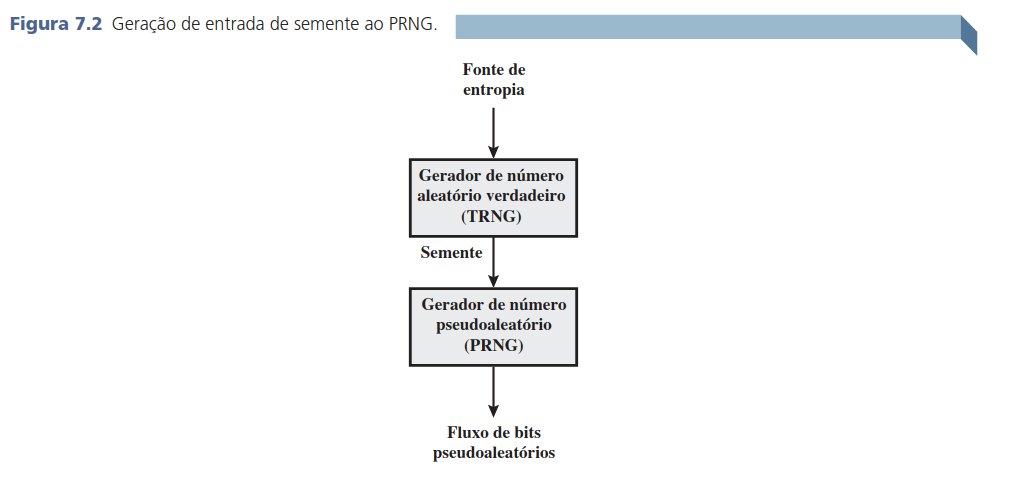
\includegraphics[width=0.9\linewidth]{Figuras/semente-entrando-prng.png}


\end{frame}

\begin{frame}{Projeto de Algoritmos de PRNG Criptográficos}
PRNGs criptográficos podem ser classificados em duas categorias principais:

\begin{itemize}
    \item \textbf{Algoritmos de propósito especial}: projetados especificamente para gerar fluxos de bits pseudoaleatórios. Alguns são usados para várias aplicações de PRNG; outros são dedicados a cifras de fluxo, como o \textbf{RC4}.
    \item \textbf{Algoritmos baseados em algoritmos criptográficos existentes}: utilizam propriedades de algoritmos criptográficos para produzir aleatoriedade.
\end{itemize}

\medskip

\textbf{Três técnicas gerais para gerar PRNGs criptograficamente fortes:}
\begin{itemize}
    \item \textbf{Cifras de bloco simétricas} 
    \item \textbf{Cifras assimétricas} 
    \item \textbf{Funções de hash e códigos de autenticação de mensagem} 
\end{itemize}

\medskip
Essas técnicas podem ser combinadas e reutilizadas de forma prática, aproveitando algoritmos já existentes em sistemas de encriptação e autenticação.
\end{frame}

%------

\begin{frame}{Fontes de Entropia em TRNGs}
\textbf{Geradores de números aleatórios verdadeiros (TRNGs) utilizam fontes não determinísticas:}
\begin{itemize}
    \item Medem processos naturais imprevisíveis, como:
    \begin{itemize}
        \item Detectores de pulso de radiação ionizante.
        \item Tubos de descarga de gás.
        \item Capacitores com escape.
    \end{itemize}
    \item Exemplos comerciais e de pesquisa:
    \begin{itemize}
        \item Chip da Intel: captura ruído térmico, amplificando voltagem de resistores não condutíveis.
        \item \textbf{LavaRnd}: projeto de código aberto que gera números verdadeiramente aleatórios usando câmeras baratas e CCD saturado como fonte caótica. \href{http://www.lavarnd.org/}{\textcolor{blue}{Link}}
    \end{itemize}
    \item O software processa as amostras e produz números aleatórios em vários formatos.
\end{itemize}
\end{frame}

\begin{frame}{Fontes de Aleatoriedade em Computadores (RFC 4086)}
\textbf{Possíveis fontes de aleatoriedade para gerar sequências verdadeiramente aleatórias:}

\begin{itemize}
    \item \textbf{Entrada de som/vídeo:} 
    \begin{itemize}
        \item Microfone sem entrada ou câmera tampada produz ruído térmico.
        \item Digitalização fornece bits aleatórios de qualidade razoável.
    \end{itemize}
    \item \textbf{Unidades de disco:}
    \begin{itemize}
        \item Pequenas flutuações aleatórias na rotação devido à turbulência do ar.
        \item Medições de tempo de busca geram dados aleatórios, embora correlacionados.
        \item Processamento adequado pode extrair excelentes bits aleatórios (ex.: 100 bits/min em discos antigos).
    \end{itemize}
    \item Serviço on-line \href{http://random.org}{\textcolor{blue}{random.org}} que pode oferecer sequências aleatórias pela Internet.

    \item Exemplo de TCC no tema de geração de números aleatórios: \href{https://lume.ufrgs.br/handle/10183/251751}{\textcolor{blue}{Link}}
\end{itemize}
\end{frame}


\begin{frame}{Geradores de números aleatórios e pseudoaleatórios}

\centering
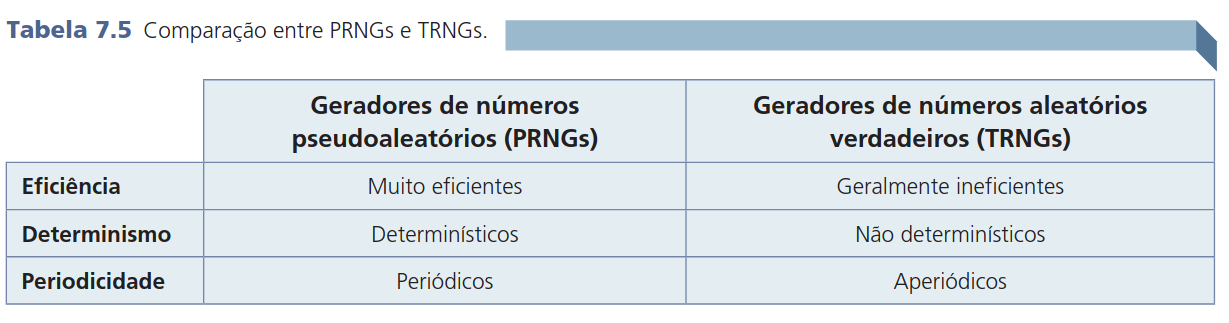
\includegraphics[width=0.9\linewidth]{Figuras/tabelaprngtrng.png}


\end{frame}

\begin{frame}{PRNGs: Números Pseudoaleatórios Determinísticos}
\textbf{Características principais dos PRNGs:}

\begin{itemize}
    \item \textbf{Eficiência:} podem gerar muitos números rapidamente, adequado para aplicações que exigem grandes quantidades de números pseudoaleatórios.
    \item \textbf{Determinismo:} a mesma sequência pode ser reproduzida se a condição inicial (semente) for conhecida.
    \item \textbf{Periodicidade:} as sequências eventualmente se repetem, mas PRNGs modernos possuem períodos tão longos que são irrelevantes para a maioria das aplicações.
\end{itemize}

\end{frame}

\begin{frame}{TRNGs: Números Aleatórios Verdadeiros}
\textbf{Características principais dos TRNGs:}

\begin{itemize}
    \item \textbf{Eficiência:} geralmente mais lentos que PRNGs, podendo ser um gargalo em aplicações que exigem muitos números aleatórios por segundo.
    \item \textbf{Não determinísticos:} a mesma sequência não pode ser reproduzida de forma garantida.
    \item \textbf{Sem periodicidade:} não possuem ciclo repetitivo, diferentemente dos PRNGs.
    \item \textbf{Aplicações críticas:} úteis em contextos onde imprevisibilidade máxima é necessária, como criptografia bancária ou nacional.
\end{itemize}

\end{frame}

\begin{frame}{Propensão em TRNGs e Algoritmos Antipropensão}
\textbf{Propensão:} um TRNG pode gerar uma saída tendenciosa, com mais uns ou zeros.

\textbf{Soluções:}
\begin{itemize}
    \item Aplicação de \textbf{algoritmos antipropensão} para reduzir ou eliminar a tendência.
    \item Uso de \textbf{funções de hash} (MD5, SHA-1) para misturar blocos de bits:
        \begin{itemize}
            \item Blocos de $m \ge n$ bits de entrada processados para gerar $n$ bits de saída.
            \item Mistura de entradas de diferentes fontes de hardware.
        \end{itemize}
    \item Sistemas operacionais oferecem mecanismos embutidos:
        \begin{itemize}
            \item Linux: combina atividade do mouse/teclado, E/S de disco e interrupções. A saída aleatória passa por SHA-1 antes de ser fornecida.

            \item \href{https://man.archlinux.org/man/urandom.4.en}{\textcolor{blue}{Leia}}
        \end{itemize}
\end{itemize}

\end{frame}

\begin{frame}{Gerador de Números Aleatórios Digitais da Intel (DRNG)}
\textbf{Contexto:} TRNGs tradicionais eram usados apenas para gerar pequenas quantidades de bits aleatórios devido à baixa taxa de produção.

\textbf{Intel DRNG:} primeiro TRNG comercial com taxa de produção comparável a PRNGs, disponível em chips multicore desde 2012.

\textbf{Destaques:}
\begin{itemize}
    \item \textbf{Implementação totalmente em hardware:} maior segurança e velocidade comparada a soluções baseadas em software.
    \item \textbf{Integração no chip multicore:} elimina atrasos de E/S encontrados em outros TRNGs.
\end{itemize}

\end{frame}

\begin{frame}{Intel DRNG}

\centering
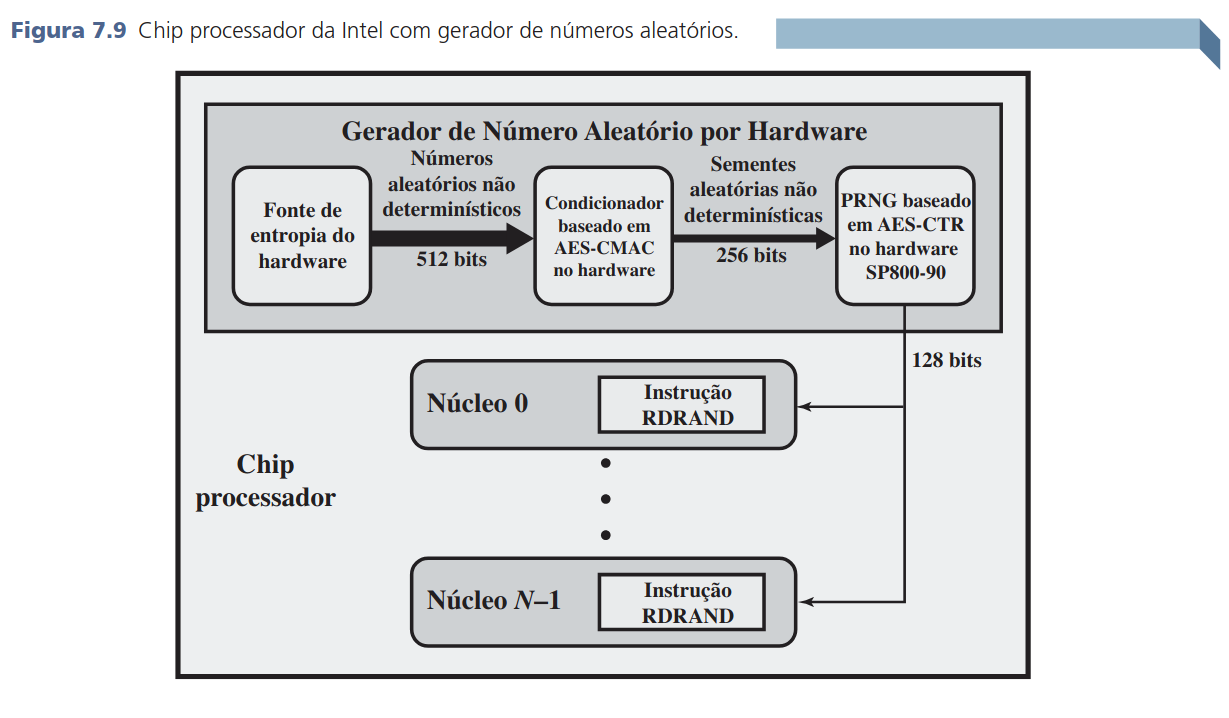
\includegraphics[width=0.9\linewidth]{Figuras/gerador-numero-aleatorio-intel.png}


\end{frame}


\begin{frame}{Visão Geral do Intel DRNG}

    O DRNG é uma arquitetura de \textbf{três estágios}:
    \begin{enumerate}
        \item \textbf{Fonte de Entropia}: Gera bits aleatórios a partir do ruído térmico.
        \item \textbf{Condicionador}: Remove qualquer viés ou correlação residual.
        \item \textbf{PRNG}: Expande a aleatoriedade para maior throughput.
    \end{enumerate}
\end{frame}


\begin{frame}{Estágio 1: Fonte de Entropia (O Núcleo Aleatório)}
    
            \begin{itemize}
                \item \textbf{Núcleo}: Dois inversores (portas NOT).
                \item Possui dois estados estáveis lógicos.
                \item Pulsos de \textit{clock} forçam ambos para um \textbf{estado metaestável} indeterminado.
                \item O \textbf{ruído térmico} aleatório dentro dos transistores decide para qual estado estável o circuito irá decair.
                \item Este decaimento é fundamentalmente \textbf{imprevisível}.
            \end{itemize}
    \vspace{0.5cm}
    \begin{block}{Desempenho}
        Gera bits a uma taxa de \textbf{4 Gbps} (Gigabits por segundo). A saída é colhida em blocos de \textbf{512 bits}.
    \end{block}
\end{frame}

\begin{frame}{Estágio 2: Condicionamento com CMAC}
    \begin{itemize}
        \item \textbf{Problema}: A saída do estágio 1 pode ter \textbf{viés} ou ter \textbf{correlações} sutis.
        \item \textbf{Solução}: Um condicionador criptográfico.
        \item \textbf{Função}: CBC-MAC (CMAC), conforme padrão NIST SP 800-38B.
    \end{itemize}



    \begin{block}{Como funciona?}
        \begin{itemize}
            \item Os 512 bits do Estágio 1 são criptografados em modo \textbf{CBC} usando o algoritmo AES.
            \item Apenas o \textbf{último bloco cifrado} (o MAC) é tomado como saída.
            \item Esta etapa \"distila\" a entropia, produzindo \textbf{256 bits} verdadeiramente aleatórios e não enviesados por bloco.
        \end{itemize}
    \end{block}
\end{frame}

\begin{frame}{Estágio 3: Geração em Alta Velocidade (PRNG)}
    \begin{itemize}
        \item \textbf{Problema}: Mesmo a 4 Gbps, a entropia pura não é suficientemente rápida para todas as aplicações modernas.
        \item \textbf{Solução}: Usar os bits aleatórios do Estágio 2 como \textbf{semente} para um PRNG.
    \end{itemize}

    \begin{block}{Algoritmo: CTR\_DRBG}
        \textbf{Counter Mode Deterministic Random Bit Generator}
        \begin{itemize}
            \item \textbf{Semente}: Os 256 bits do Estágio 2.
            \item \textbf{Funcionamento}: Criptografa um contador incremental usando AES.
            \item \textbf{Saída}: Gera números pseudoaleatórios de \textbf{128 bits}.
            \item \textbf{Segurança}:  Sem a semente, é computacionalmente inviável prever a saída.
        \end{itemize}
    \end{block}

    \begin{exampleblock}{Vantagem}
        A partir de uma única semente de 256 bits, o PRNG pode gerar \textbf{muitos} blocos de 128 bits, ultrapassando a taxa da fonte de entropia (\textbf{$>$3 Gbps}). Um limite de \textbf{511 amostras} é definido por semente para garantir a segurança antes de uma nova ressementeação.
    \end{exampleblock}
\end{frame}

\begin{frame}{Interface com o Software: A Instrução RDRAND}
    \begin{itemize}
        \item A saída final do DRNG (seja do Estágio 2 ou 3) é disponibilizada para todos os núcleos do processador.
        \item Acesso via uma instrução de assembly dedicada: \textbf{RDRAND}.
    \end{itemize}

    \begin{block}{Instrução RDRAND}
        \texttt{RDRAND reg} \\
        onde \texttt{reg} pode ser um registrador de 16, 32 ou 64 bits (\texttt{AX}, \texttt{EAX}, \texttt{RAX}).
        \begin{itemize}
            \item A instrução busca um valor aleatório do tamanho solicitado.
            \item Define a flag de \emph{carry} (CF=1) em caso de sucesso.
            \item Software deve verificar o \emph{carry} para garantir que obteve um valor aleatório válido.
        \end{itemize}
    \end{block}


   \href{https://www.intel.com/content/www/us/en/developer/articles/guide/intel-digital-random-number-generator-drng-software-implementation-guide.html}{\textcolor{blue}{Leitura interessante - Link da Intel}}
\end{frame}

\begin{frame}{Intel DRNG: Estrutura lógica}

\centering
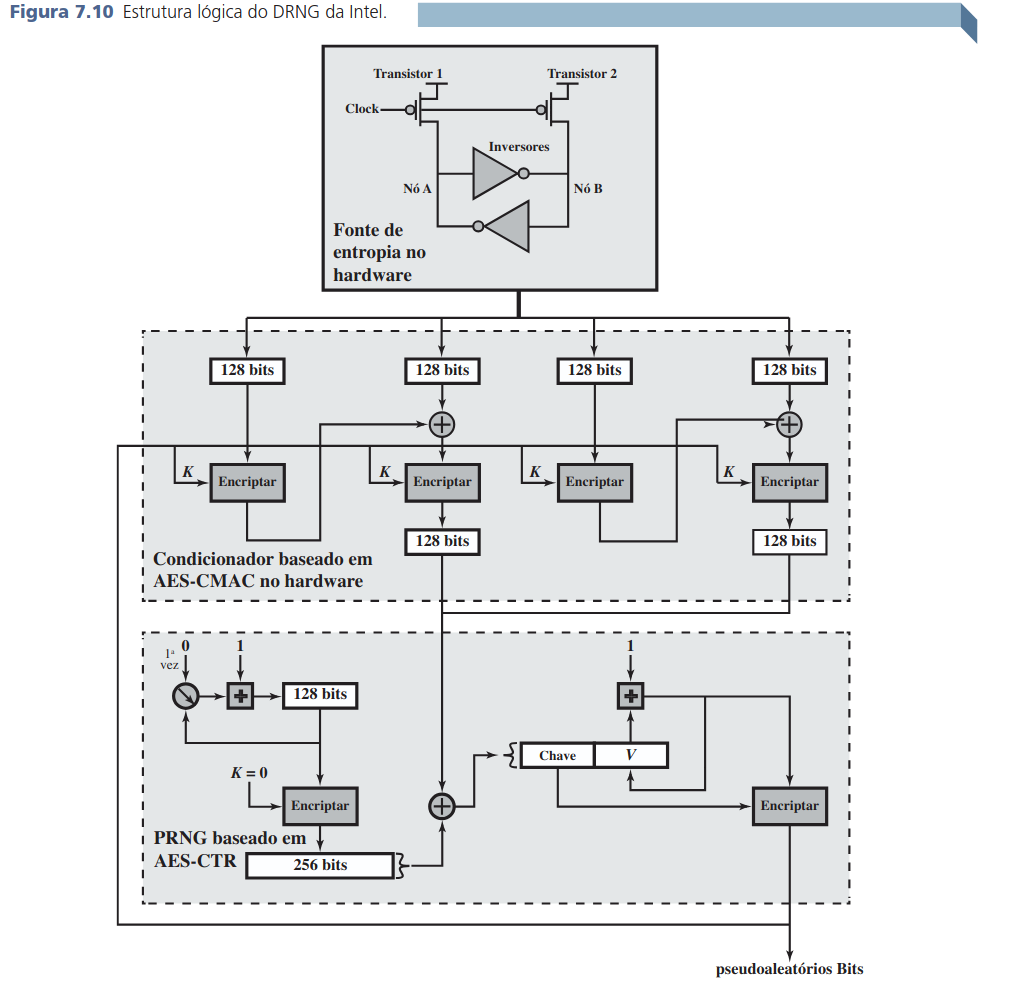
\includegraphics[width=0.55\linewidth]{Figuras/estrutura-logica-drng-intel.png}




\end{frame}

\begin{frame}[fragile]{Código executando o rdrand}
\tiny
    \begin{verbatim}
section .text
    global _start

_start:
    rdrand rcx          ; Bota valor aleatorio no registrador RCX - 64 bits
    jnc .exit           ; Vai pular se NÃO tiver o carry flag (CF = 0)

    ; Escreve os 64 bits diretamente na saída padrao (terminaL)
    push rcx            ; coloca os 64 bits na stack
    mov rax, 1          ; Fala qual e a operacao - sys_write
    mov rdi, 1          ; Fala aonde que vai escrever - stdout
    mov rsi, rsp        ; Fala onde que é pra ler - aponta leitura para os dados na stack (rsp é o stack pointer)
    mov rdx, 8          ; Fala a quantidade pra ler - 8 bytes (64 bits)
    syscall

    add rsp, 8          ; Joga o stack pointer 8 bytes para cima - ou seja, limpa a stack

.exit:
    mov rax, 60         ; Fala qual que e a operacao - no caso sys_exit
    xor rdi, rdi        ; Bota zero no rdi - exit(0)
    syscall
    \end{verbatim}
\end{frame}

\begin{frame}[fragile]{Compilando o código com rdrand}
\begin{verbatim}
$nasm -f elf64 rdrand_bin.asm -o rdrand_bin.o
$ld rdrand_bin.o -o rdrand_bin
$ ./rdrand_bin | hexdump -C

\end{verbatim}
    
\end{frame}